% \documentclass[a4paper,12pt]{article}

% % Paquetes básicos
% \usepackage[utf8]{inputenc}
% \usepackage[T1]{fontenc}
% \usepackage[spanish]{babel}
% \usepackage{graphicx}
% \usepackage{xcolor}
% \usepackage{lipsum}
% \usepackage{geometry}
% \geometry{top=3cm, bottom=3cm, left=2.5cm, right=2.5cm}

% % Paquetes para diseño
% \usepackage{titlesec}
% \usepackage{fancyhdr}
% \usepackage{amsmath}
% \usepackage{amssymb}
% \usepackage{hyperref}

% % Paquetes para el entorno lstlisting
% \usepackage{listings}
% \usepackage{inconsolata}

% % Paquete para fondo
% \usepackage{background}

% % Configuración de lstlisting
% \lstset{
%     language=Python,
%     basicstyle=\ttfamily\small,
%     keywordstyle=\color{blue}\bfseries,
%     stringstyle=\color{teal},
%     commentstyle=\color{gray}\itshape,
%     numbers=left,
%     numberstyle=\tiny\color{gray},
%     backgroundcolor=\color{black!5},
%     frame=single,
%     rulecolor=\color{black!50},
%     breaklines=true,
%     captionpos=b,
%     showstringspaces=false
% }

% % Configuración de título
% \titleformat{\section}{\normalfont\Large\bfseries}{\thesection}{1em}{}
% \usepackage{mathpazo}

% %encabezado y pie de página nivel profesional
% \usepackage{fancyhdr}
% \pagestyle{fancy}
% \fancyhf{}
% \fancyhead[L]{\leftmark}
% \fancyhead[R]{\rightmark}
% \fancyfoot[C]{\thepage}
% \fancyfoot[R]{\textbf{       (UGR)} \today}



% % Información del documento
% \title{
%     \vspace{-2cm}
%     
\includegraphics[width=0.3\textwidth]{images/fccee.jpg} \\ % Cambia el logo si es necesario
%     \LARGE Ingeniería Informática + ADE\\
%     \large Universidad de Granada (UGR)\\[1cm]
% }
% \author{\textbf{Autor:} Ismael Sallami Moreno}
% \date{\textbf{Asignatura:} Resolución de los Ejercicios Propuestos Reueltos Tema 5: Inmovilizaciones materiales}

% % Configuración del fondo
% \backgroundsetup{
%     scale=1,
%     color=black,
%     opacity=0.2,
%     angle=0,
%     position=current page.south,
%     vshift=0pt,
%     hshift=0pt,
%     contents={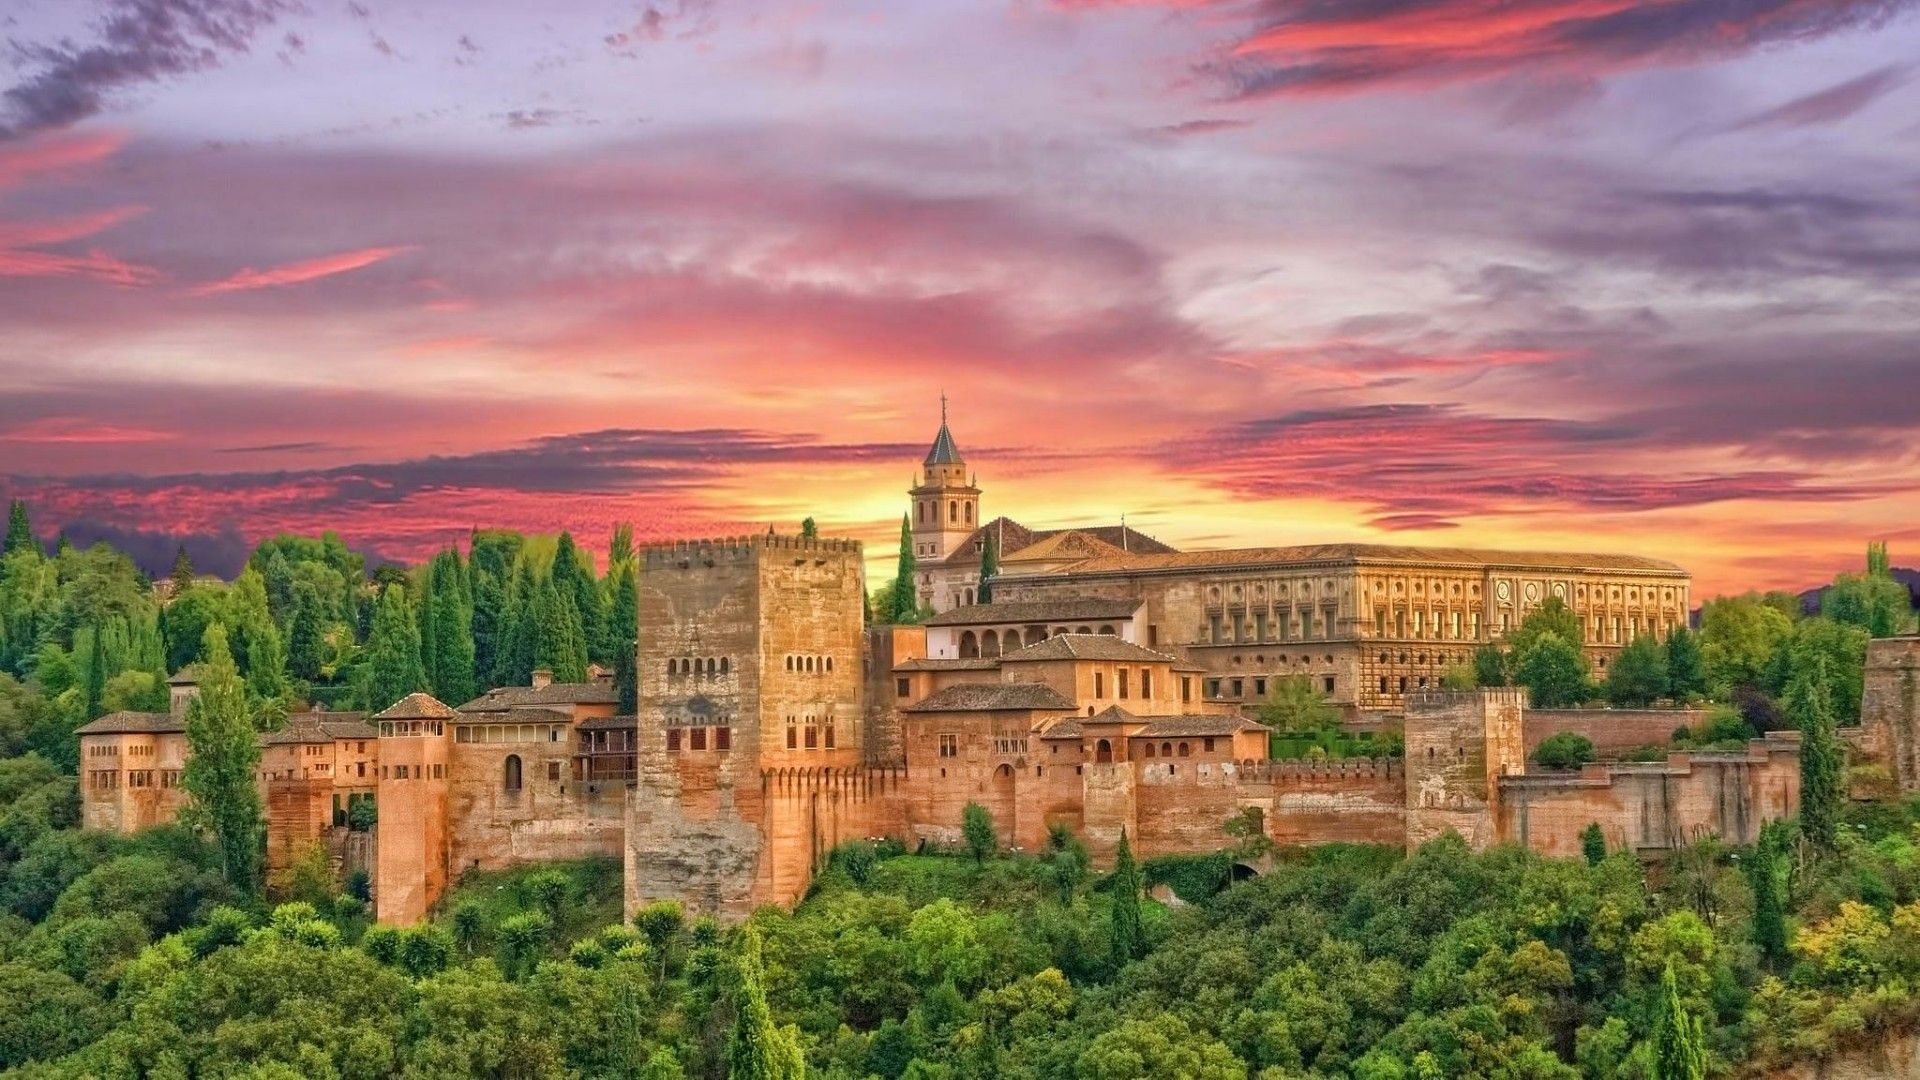
\includegraphics[width=\paperwidth,height=\paperheight,keepaspectratio]{images/granada.jpg}}
% }


\documentclass[a4paper,12pt]{article}

% Paquetes básicos
\usepackage[utf8]{inputenc}
\usepackage[T1]{fontenc}
\usepackage[spanish]{babel}
\usepackage{graphicx}
\usepackage{xcolor}
\usepackage{lipsum}
\usepackage{geometry}
\geometry{top=3cm, bottom=3cm, left=2.5cm, right=2.5cm}

% Paquetes para diseño
\usepackage{titlesec}
\usepackage{fancyhdr}
\usepackage{amsmath}
\usepackage{amssymb}
\usepackage{hyperref}
\usepackage{tcolorbox}
\usepackage{float}

% Paquetes para el entorno lstlisting
\usepackage{listings}
\usepackage{inconsolata}

\usepackage{tocbibind} % Para incluir subsubsubsections en el índice
\usepackage{titlesec}  % Para ajustar la numeración de las secciones
\setcounter{tocdepth}{5} % Ajusta la profundidad del índice
\setcounter{secnumdepth}{5} % Ajusta la profundidad de la numeración

% Configuración de la numeración para \paragraph
\titleformat{\paragraph}
{\normalfont\normalsize\bfseries}{\theparagraph}{1em}{}
\titlespacing*{\paragraph}{0pt}{3.25ex plus 1ex minus .2ex}{1.5ex plus .2ex}

% Paquete para fondo
\usepackage{background}

\newcommand{\fec}{31/12/}
\newcommand{\AIM}{681 Amortización del inmovilizado material }
\newcommand{\AAMAQ}{2813 Amortización acumulada de maquinaria }
\newcommand{\valorrecuperable}{Valor recuperable = max\{valor neto realizable, valor en uso\} =}
\newcommand{\PDI}{691 Pérdidas por deterioro de inmovilizado material}
\newcommand{\DVM}{2913 Deterioro del valor de la maquinaria }
\newcommand{\RDIM}{791 Reversión deterioro inmovilizado material}
\newcommand{\VC}{Valor contable = }
\newcommand{\PPIM}{671 Pérdidas procedentes del inmovilizado material}
\newcommand{\bancos}{572 Bancos cuenta corriente}
\newcommand{\cuotaamort}{Cuota de amortización = }
\newcommand{\enajenacion}{543 Créditos a corto plazo por enajenación del inmovilizado}
\newcommand{\benefIM}{771 Beneficios procedentes del inmovilizado material}
\usepackage{amsmath}
\newcommand{\myequation}[2]{\ensuremath{\frac{#1}{#2}}}
\newcommand{\flechita}{$\rightarrow$}

% Configuración de lstlisting
\lstset{
    language=Python,
    basicstyle=\ttfamily\small,
    keywordstyle=\color{blue}\bfseries,
    stringstyle=\color{teal},
    commentstyle=\color{gray}\itshape,
    numbers=left,
    numberstyle=\tiny\color{gray},
    backgroundcolor=\color{black!5},
    frame=single,
    rulecolor=\color{black!50},
    breaklines=true,
    captionpos=b,
    showstringspaces=false
}

% Configuración de título
\titleformat{\section}{\normalfont\Large\bfseries}{\thesection}{1em}{}

% Información del documento
\title{
    \vspace{-2cm}
    
\includegraphics[width=0.3\textwidth]{images/fccee.jpg} \\ % Cambia el logo si es necesario
    \LARGE Ingeniería Informática + ADE\\
    \large Universidad de Granada (UGR)\\[1cm]
}
\author{\textbf{Autor:} Ismael Sallami Moreno}
\date{\textbf{Asignatura:} Resolución de los Ejercicios Propuestos Reueltos Tema 5: Inmovilizaciones materiales
}
\usepackage{mathpazo}
\usepackage{fancyhdr}
\pagestyle{fancy}
\fancyhf{}
\fancyhead[L]{\leftmark}
\fancyhead[R]{\rightmark}
\fancyfoot[C]{\thepage}
\fancyfoot[R]{\textbf{       (UGR)} \today}
\usepackage{enumitem}

\usepackage{tcolorbox}

% Configuración del fondo
\backgroundsetup{
    scale=1,
    color=black,
    opacity=0.2,
    angle=0,
    position=current page.south,
    vshift=0pt,
    hshift=0pt,
    contents={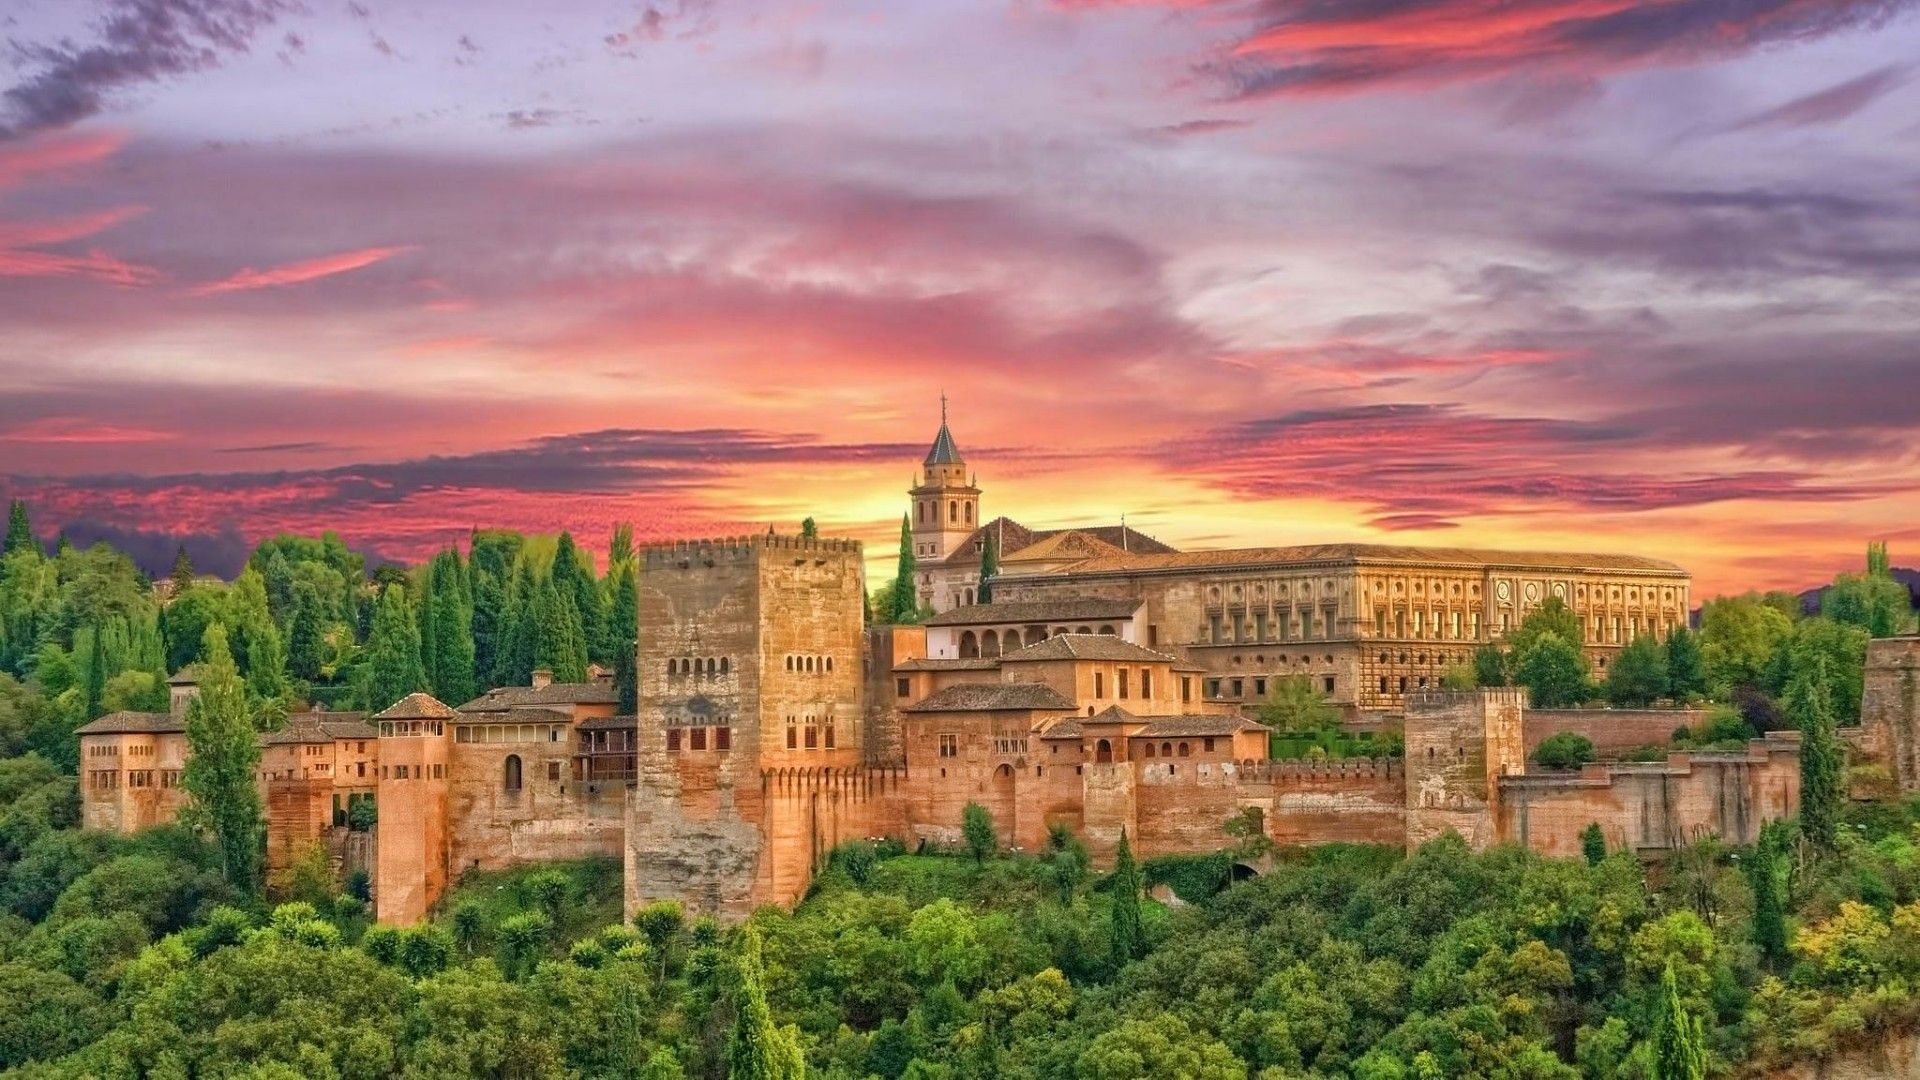
\includegraphics[width=\paperwidth,height=\paperheight,keepaspectratio]{images/granada.jpg}}
}

% Inicio del documento
\begin{document}

% Portada
\maketitle
\thispagestyle{empty}

\begin{center}
    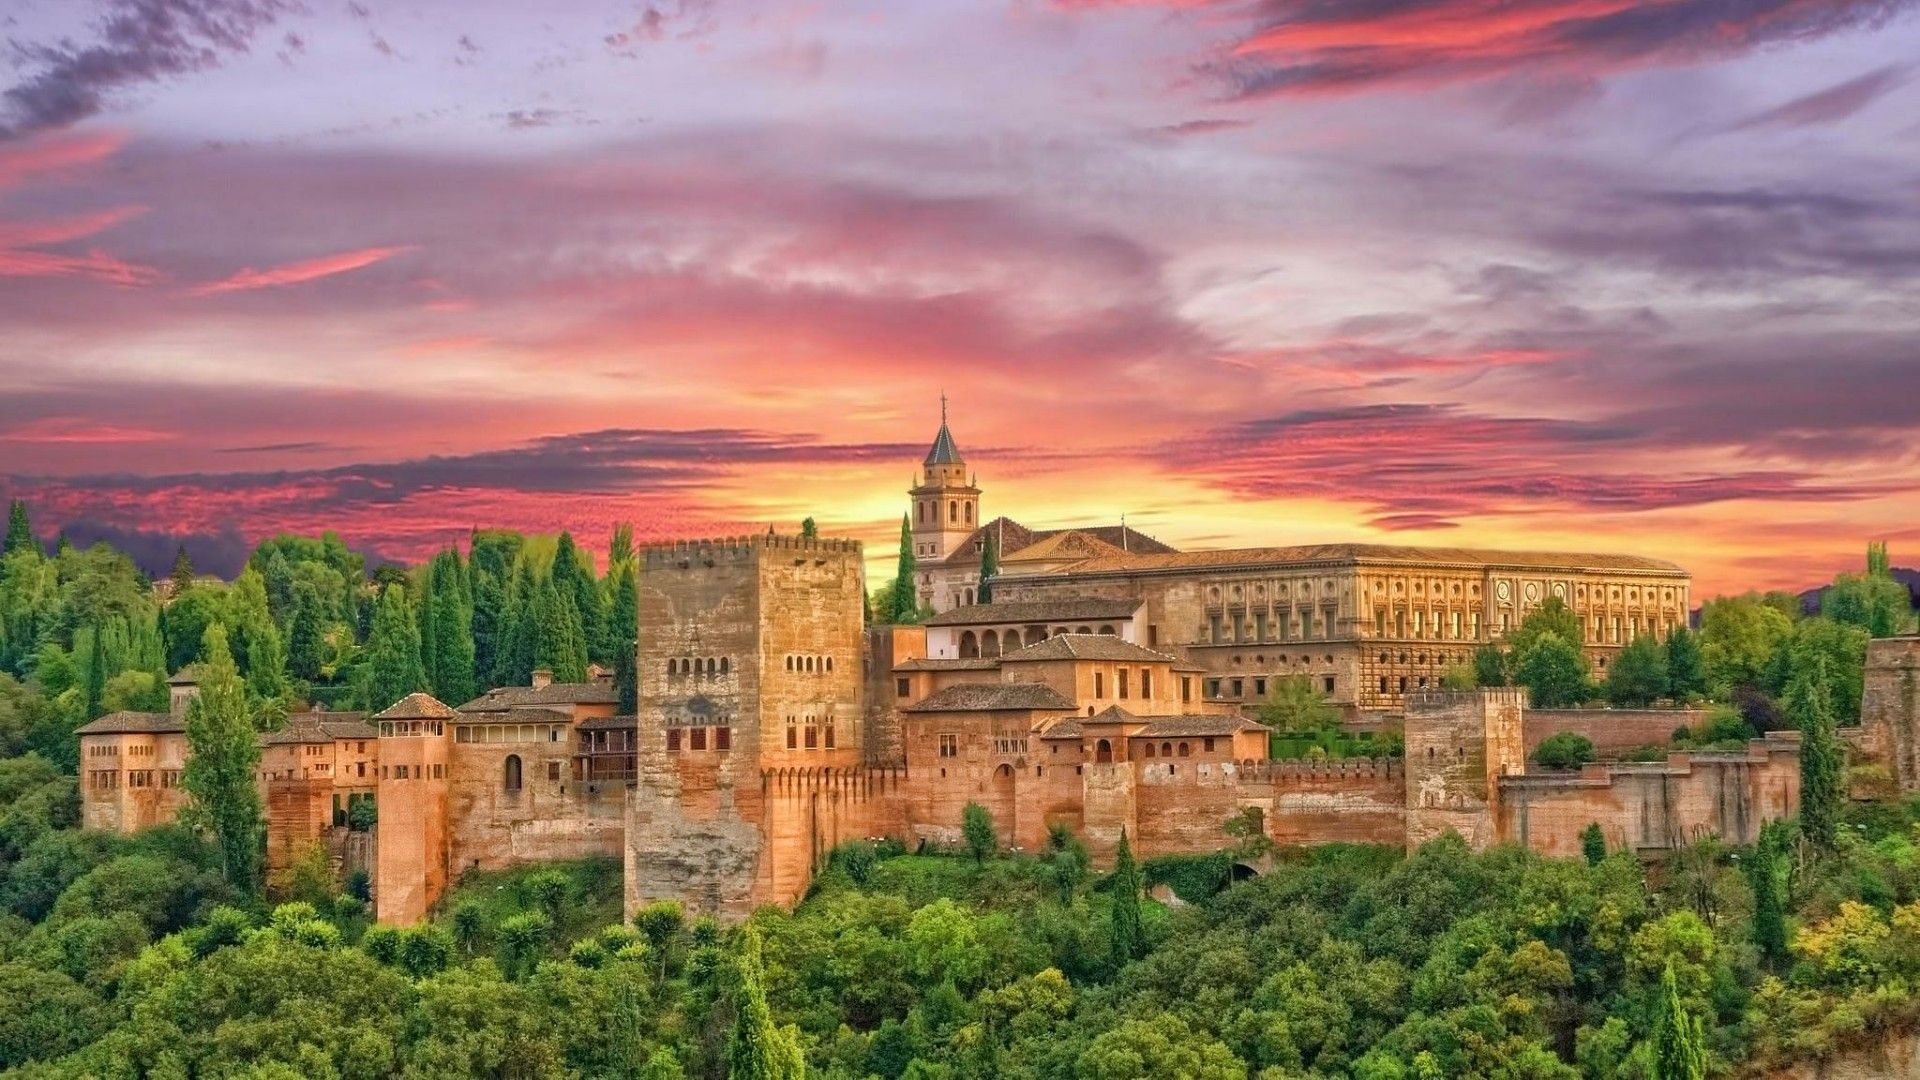
\includegraphics[width=\textwidth,height=0.4\textheight,keepaspectratio]{images/granada.jpg} \\ % Añade tu imagen de fondo
    \vfill
\end{center}

\newpage

% Índice (opcional)
\tableofcontents
\newpage

\section{Ejercicio 1}

\begin{table}[H]
    \centering
    \begin{tabular}{|p{3cm}|p{6cm}|p{3cm}|}
    \hline
    \textbf{DEBE} & \textbf{Compra de inmovilizados a 1/07/2020} & \textbf{HABER} \\
    \hline
    $39500+29400=68900$& 233 Maquinaria en montaje& \\
    \hline
    14469 & 472 HP IVA S& \\
    \hline
    & 572 bancos & 83369\\
    \hline
    \end{tabular}
\end{table}

\begin{table}[H]
    \centering
    \begin{tabular}{|p{3cm}|p{6cm}|p{3cm}|}
    \hline
    \textbf{DEBE} & \textbf{Amortización de los inmovilizados el 31/12/2020} & \textbf{HABER} \\
    \hline
    & No procede asiento contable debido a que ninguna máquina adquirida ha terminado el proceso de montaje& \\
    \hline
    \end{tabular}
\end{table}

\begin{itemize}
    \item Solo se nos pide de la máquinaria especial asumiendo que los gastos de la instalación de los equipos industriales ya han sido contabilizados.
\end{itemize}

\begin{table}[H]
    \centering
    \begin{tabular}{|p{3cm}|p{6cm}|p{3cm}|}
    \hline
    \textbf{DEBE} & \textbf{Asiento por la máquina especial el 01/12/2021 al entrar en funcionamiento} & \textbf{HABER} \\
    \hline
    $29400+300 = 30000$ & 213 maquinaria & \\
    \hline
    $600*0,21 = 126$ & 472 HP IVA s & \\
    \hline
    & 572 bancos & 726 \\
    \hline
    & 233 Maquinaria en montaje & 29.400 \\
    \hline
    \end{tabular}
\end{table}

\section{Ejercicio 2}

\begin{table}[H]
    \centering
    \begin{tabular}{|p{3cm}|p{6cm}|p{3cm}|}
    \hline
    \textbf{DEBE} & \textbf{Amortización de la maquinaria \fec2020} & \textbf{HABER} \\
    \hline
    $\frac{1000000}{10}=100000 $& \AIM & \\
    \hline
    & \AAMAQ & 100000\\
    \hline
    \end{tabular}
\end{table}

Deterioro de valor:
\begin{itemize}
    \item \AAMAQ  es $100000*5=500000$ debido a los 5 años desde 2016 hasta 2020.
    \item Valor contable $= 1000000-500000=500000$
    \item Valor recuperable = max\{valor neto realizable, valor en uso\} = max\{450000\} (nos lo dice directamente) = 450000
    \item Deterioro = 600000-500000 = 50000 (Debemos de dotar las cuentas de pérdidas y ganancias)
\end{itemize}
\begin{table}[H]
    \centering
    \begin{tabular}{|p{3cm}|p{6cm}|p{3cm}|}
    \hline
    \textbf{DEBE} & \textbf{Deterioro de valor de la maquinaria \fec2020} & \textbf{HABER} \\
    \hline
    50000& \PDI & \\
    \hline
    & \DVM & 50000\\
    \hline
    \end{tabular}
\end{table}

\begin{itemize}
    \item Debemos de calcular la nueva cuota de Amortización = 1.000.000 - 500.000 - 50.0000 = 650.000 entre los restantes años (llevamos 5), nos quedan otros 5 = $\frac{450000}{5}$ = 90.000
\end{itemize}

\begin{table}[H]
    \centering
    \begin{tabular}{|p{3cm}|p{6cm}|p{3cm}|}
    \hline
    \textbf{DEBE} & \textbf{Amortización de la maquinaria \fec2021} & \textbf{HABER} \\
    \hline
    90.000& \AIM & \\
    \hline
    & \AAMAQ & 90.000 \\
    \hline
    \end{tabular}
\end{table}

Deterioro de valor:
\begin{itemize}
    \item \AAMAQ es 500.000 + 90.000 + 90.000 = 680.000
    \item Valor contable = 1.000.000 - 680.000 = 320.000
    \item Valor recuperable = 350.000 a \fec2022
    \item Deterioro = 350.000 - 320.000 = 30.000 (\textit{No hay deterioro,debemos de revertir})
\end{itemize}

\begin{tcolorbox}[colback=blue!5!white, colframe=blue!75!black, title=Deterioro de valor]  
    IMPORTANTE: debemos de revertir el deterioro anterior
\end{tcolorbox}

\begin{table}[H]
    \centering
    \begin{tabular}{|p{3cm}|p{6cm}|p{3cm}|}
    \hline
    \textbf{DEBE} & \textbf{Deterioro de valor a \fec2022} & \textbf{HABER} \\
    \hline
    90.000& \AIM & \\
    \hline
    & \AAMAQ & 90.000\\
    \hline
    30.000& \DVM & \\
    \hline
    & 791 Reversión del deterioro del inmovilizado material & 30.000\\
    \hline
    \end{tabular}
\end{table}

\section{Ejercicio 3}

\begin{itemize}
    \item Cuota de amortización = $\frac{2000000}{16} = 125000$
    \item Cierre del ejercicio de 2020, la cuenta de 281 Amortización acumulada del inmovilizado material es de 125000·6 = 750000
    \item \valorrecuperable siendo el neto realizable 1.200.000 - 50.000 = 1.150.000 y el valor en uso 1.100.000 = 1.150.000
    \item \VC 2.000.000 - 750.000 = 1.250.000
    \item Deterioro = 1.250.000 - 1.150.000 = 100.000
\end{itemize}

\begin{table}[H]
    \centering
    \begin{tabular}{|p{3cm}|p{6cm}|p{3cm}|}
    \hline
    \textbf{DEBE} & \textbf{Deterioro del inmovilizado a \fec2020} & \textbf{HABER} \\
    \hline
    100.000& \PDI & \\
    \hline
    & 2918 Deterioro de valor de elementos de transporte & 100.000\\
    \hline
    \end{tabular}
\end{table}

\begin{itemize}
    \item El 1 de abril de 2021 decide venderlo
    \item Precio de venta = 1.400.000 + 21 \% IVA = 1.694.000   
    \item la cantidad la cobrará dentro de 3 meses
    \item Debemos de calcular la Amortización hasta esta fecha:
    \begin{itemize}
        \item 2.000.000 - 125.000·6 - 100.000 = 1.150.000
        \item los años restates son 10 $\rightarrow \frac{1150000}{10} = 115000$
        \item Cuota de Amortización a partir de ahora es = 115.000
    \end{itemize}
\end{itemize}
\begin{table}[H]
    \centering
    \begin{tabular}{|p{3cm}|p{6cm}|p{3cm}|}
    \hline
    \textbf{DEBE} & \textbf{Todas las operaciones a 01/04/2021} & \textbf{HABER} \\
    \hline 
    1.694.000 & \textit{\enajenacion}& \\
    \hline
    750.000 + 115.000·$\frac{3}{12} =$ 778.750 & 281 Amortización acumulada del inmovilizado material& \\
    \hline
    100.000&2918 Deterioro de valor de elementos de transporte&\\
    \hline
    & 213 maquinaria, pensamos que ese barco forma parte de la maquinaria de la empresa& 2.000.000 \\
    \hline
    & 477 HP IVA r& 294.000\\
    \hline
    & \benefIM & $2472750 - 2294000 - 100000= 78750$\\
    \hline
    \end{tabular}
\end{table}


\section{Ejercicio 4}

\begin{tcolorbox}[colback=red!5!white, colframe=yellow!75!black, title=NOTA]  
    \textbf{IMPORTANTE:} Suponemos que el asiento de la máquina en montaje ya ha sido realizado y los demás pagos de transportes y de instalación también. Además, suponemos que el IVA ya va incluido en el precio de la máquina.
    
\end{tcolorbox}
\begin{tcolorbox}[colback=red!5!white, colframe=yellow!75!black, title=NOTA]  
    \textbf{IMPORTANTE:} El pago se realiza el 1 de junio, en el primer asiento que nos piden aún queda 1 mes, por lo que no contabilizamos ese cobro aún. Cabe destacar que en el asiento que hemos supuesto \textit{hay que abonar la cuenta de deuda 523 Proveedores de inmovilizado a corto plazo} por 200.000 + 21\% IVA = 242.000
    
\end{tcolorbox}

\begin{table}[H]
    \centering
    \begin{tabular}{|p{3cm}|p{6cm}|p{3cm}|}
    \hline
    \textbf{DEBE} & \textbf{operaciones de la maquinaria a 1 de junio de 2020} & \textbf{HABER} \\
    \hline
    210.000& 213 Máquinaria& \\
    \hline
    & 233 Máquina en montaje& 205.000\\
    \hline
    & 572 Bancos& 5.000 (de la calibración)\\
    \hline
    \end{tabular}
\end{table}

\begin{tcolorbox}[colback=red!5!white, colframe=yellow!75!black, title=NOTA]  
    \textit{Si hubiese IVA, deberíamos de anotarlo en la cuenta 477, en este caso suponemos que no hay debido a que el enunciado no expone nada sobre ello.}
    
\end{tcolorbox}

\begin{itemize}
    \item \valorrecuperable 155.000
    \item cuota de Amortización = $\frac{210000}{10} = 21.000$
    \item Hasta \fec2020 hay 7 meses $\rightarrow $ 21.000·7/12 = 12.250
    \item 2021 = 21.000
    \item 2022 = 21.000
    \item \VC = 210.000 - 12.250 - 21.000 - 21.000 = 155.750
    \item Deterioro = 155.750 - 155.000 = 750
\end{itemize}
\begin{table}[H]
    \centering
    \begin{tabular}{|p{3cm}|p{6cm}|p{3cm}|}
    \hline
    \textbf{DEBE} & \textbf{deterioro de la máquina a \fec2022} & \textbf{HABER} \\
    \hline
    750& \PDI& \\
    \hline
    & \DVM & 750\\
    \hline
    \end{tabular}
\end{table}

\begin{itemize}
    \item a \fec2023 el \valorrecuperable 160.000
    \item Nueva cuota de amortización = $\frac{155000}{89 \text{ Meses restantes}} = 1741,573 \cdot 12 = 20898,88 \frac{\text{euros}}{\text{año}} $
    \item \VC a \fec2023 es 155.000 - 20898,88 = 134.101,12
    \item \valorrecuperable 160.000
    \item Como en este caso el valor recuperable es mayor que el valor contable, no hay deterioro, \textit{debemos de dotar la reversión}
    \item Debemos de calcular el límite de lo que podemos revertir, para ello:
    \begin{itemize}
        \item $\text{Valor contable}_{\text{Sin deterioro}}$ = 210.000 - 12.250 - 21.000 - 21.000 - 21.0000 = 134.750
        \item Límite de la reversión debe de ser = 134.750 - 134.101,12 = 648,88
        \item \textit{No podemos revertir los 750, debe de ser 648,88} 
    \end{itemize}
\end{itemize}

\begin{table}[H]
    \centering
    \begin{tabular}{|p{3cm}|p{6cm}|p{3cm}|}
    \hline
    \textbf{DEBE} & \textbf{correrción valorativa reversible de la maquinaria} & \textbf{HABER} \\
    \hline
    648,88 & \DVM  & \\
    \hline
    & \RDIM& 648,88\\
    \hline
    \end{tabular}
\end{table}

\begin{itemize}
    \item Calculamos la nueva cuota de Amortización:
    \begin{itemize}
        \item a \fec2024 \VC 134.101,12 + 688,88 = 134.750
        \item los años restantes son 3 años + 7 meses - 120 meses = quedan 77 meses (años con decimales)
        \item La nueva cuota de amortización es $\frac{134750}{77} = 1750$ por mes = 21000 al año
    \end{itemize}
\end{itemize}

\begin{table}[H]
    \centering
    \begin{tabular}{|p{3cm}|p{6cm}|p{3cm}|}
    \hline
    \textbf{DEBE} & \textbf{ A \fec2024 la amortización} & \textbf{HABER} \\
    \hline
    21.000 & \AIM & \\
    \hline
    & \AAMAQ & 21.000\\
    \hline
    \end{tabular}
\end{table}

\section{Ejercicio 5}

\begin{itemize}
    \item Para la adquisición de la máquina debemos de tener en cuenta:
    \begin{itemize}
        \item 50.000 de la adquisición · 0,9 debido al descuento + gastos de transporte y seguro de 3.500 + ubicación y puesta en marcha de 2.500 (suponemos que los 1000 son para la formación del personal para el uso de la máquina, por lo que no incluimos esos gastos) = 51.000
    \end{itemize}
\end{itemize}
\begin{table}[H]
    \centering
    \begin{tabular}{|p{3cm}|p{6cm}|p{3cm}|}
    \hline
    \textbf{DEBE} & \textbf{adquisición de la máquina el 1/7/2020} & \textbf{HABER} \\
    \hline
    51.000& 213 maquinaria& \\
    \hline
    & \bancos & 6.000\\
    \hline
    & 523 proveedores de inmovilizado a corto plazo& 45.000\\
    \hline
    \end{tabular}
\end{table}

\begin{itemize}
    \item \cuotaamort $\frac{51000}{10}$ = 5.100
\end{itemize}

\begin{table}[H]
    \centering
    \begin{tabular}{|p{3cm}|p{6cm}|p{3cm}|}
    \hline
    \textbf{DEBE} & \textbf{Amortización a \fec2022} & \textbf{HABER} \\
    \hline
    5.100& \AIM & \\
    \hline
    & \AAMAQ & 5.100\\
    \hline
    \end{tabular}
\end{table}

\begin{itemize}
    \item \valorrecuperable siendo el valor neto realizable 36.000 y el valor en uso 30.000 = 36.000
    \item \VC = 51.000 - 5.100 · $\frac{6}{12}$ -5100 -5100 = 38.250
    \item Deterioro = 36.000 - 38.250 = 2.250
\end{itemize}

\begin{table}[H]
    \centering
    \begin{tabular}{|p{3cm}|p{6cm}|p{3cm}|}
    \hline
    \textbf{DEBE} & \textbf{deterioro de inmovilizado a \fec2022} & \textbf{HABER} \\
    \hline
    2.250& \PDI& \\
    \hline
    & \DVM & 2.250\\
    \hline
    \end{tabular}
\end{table}

\begin{itemize}
    \item Debemos de calcular la nueva cuota de amortización debido al deterioro:
    \begin{itemize}
        \item \VC = 51.000 - 5.100 · $\frac{6}{12}$ - 5.100 - 5.100 -2250 = 36.000
        \item Tiempo restante = 120 meses - 24 meses - 6 meses = 90 meses
        \item \cuotaamort \myequation{36000}{90}=   400 = 4800 al año 
    \end{itemize}
    \item  AA total a 1/3/2023 = 5100 + 5100 + 5100/2 + 4800 *\myequation{2}{12}=13.550
\end{itemize}



\begin{table}[H]
    \centering
    \begin{tabular}{|p{3cm}|p{6cm}|p{3cm}|}
    \hline
    \textbf{DEBE} & \textbf{venta de la maquinaria a 1/3/2023} & \textbf{HABER} \\
    \hline
    13.550 (contando los dos meses de 2023)& \AAMAQ & \\
    \hline
    (suponemos que cobra la mitad de 40.000) 20.000& \bancos & \\
    \hline
    20.000 & \enajenacion & \\
    \hline
    2250&\DVM &\\
    \hline
    & \benefIM &4800(\textit{haciendo la diferencia y anotando lo que falta})\\
    \hline
    & 213 Maquinaria & 51.000\\
    \hline
    &  & \\
    \hline
    \end{tabular}
\end{table}

\section{Ejercicio 6}

\begin{table}[H]
    \centering
    \begin{tabular}{|p{3cm}|p{6cm}|p{3cm}|}
    \hline
    \textbf{DEBE} & \textbf{puesta en condiciones de funcionamiento de la maquinaria el 01/04/2022} & \textbf{HABER} \\
    \hline
    300.000 + 5.000 + 20.000 (la formación no entra) = 325.000 · 1,21 = 393.250 + 5.000 = 398.250 & 213 Maquinaria & \\
    \hline
    & \bancos& 5.000\\
    \hline
    &Suponemos que el 1 de marzo se realizó el correspondiente asiento de la cuenta \textit{523 Proveedores de inmovilizado a corto plazo} & \\
    \hline
    & 233 Maquinaria en montaje& 393.250 \\
    \hline
    \end{tabular}
\end{table}

\begin{table}[H]
    \centering
    \begin{tabular}{|p{3cm}|p{6cm}|p{3cm}|}
    \hline
    \textbf{DEBE} & \textbf{01/06/2022 de la compra del solar} & \textbf{HABER} \\
    \hline
    56.000 · 1,21 = 67.760 & 210 Terrenos y bienes naturales & \\
    \hline
    & \bancos & 67.760\\
    \hline
    \end{tabular}
\end{table}
\begin{itemize}
    \item Lo que cobra la empresa es 40.000 · 1,21 = 48.400
    \item En cuanto a la Amortización no nos comenta el enunciado ningún deterior por lo que cada año se amortiza \myequation{60000}{10} = 6.000, como pasan 3 años, la Amortización es de 18.000
\end{itemize}

\begin{table}[H]
    \centering
    \begin{tabular}{|p{3cm}|p{6cm}|p{3cm}|}
    \hline
    \textbf{DEBE} & \textbf{01/04/2022 de la venta de la furgoneta} & \textbf{HABER} \\
    \hline
    24.200 & \enajenacion & \\
    \hline
    24.200 & \bancos & \\
    \hline
    6000 · 3 = 18.000 & 2818 Amortización Acumulada de elementos de transporte& \\
    \hline
    & 218 Elementos de transporte & 60.000\\
    \hline
    & 472 HP IVA r& 8.400\\
    \hline
    2.000& \PPIM & \\
    \hline
    \end{tabular}
\end{table}

\begin{tcolorbox}[colback=red!5!white, colframe=yellow!75!black, title=NOTA]
    En contabilidad, un solar comprado con fines de inversión se registra como ``Inversiones inmobiliarias'' en el balance. Si hay mejoras o construcciones en el terreno, esas sí pueden estar sujetas a amortización, pero el valor del terreno en sí no lo está.
\end{tcolorbox}

\begin{itemize}
    \item Amortizaciones:
    \begin{itemize}
        \item Maquinaria: \myequation{398250}{10} = 39.825 (No nos comentan nada de deterioro) \flechita 39.825 · \myequation{9}{12} = 29.869,75
        \item Explanación del terreno: \myequation{6000}{10} = 600 \flechita 600 · \myequation{9}{12} = 450
    \end{itemize}
\end{itemize}
\begin{table}[H]
    \centering
    \begin{tabular}{|p{3cm}|p{6cm}|p{3cm}|}
    \hline
    \textbf{DEBE} & \textbf{amortizaciones de los elementos que posee la empresa a \fec2022} & \textbf{HABER} \\
    \hline
    29.869,75 + 450 = 30.319,75 & \AIM & \\
    \hline
    & \AAMAQ& 29.869,75\\
    \hline
    &  2811 Amortización acumulada de Construcciones \textbf{ó} 2819 Amortización acumulada de otro inmovilizado material& 450 \\
    \hline
    \end{tabular}
\end{table}

\section{Ejercicio 7}
Similar a los que llevamos haciendo pero aplicando conceptos sobre el tema 4 y 5.

\section{Ejercicio 8}
Similar a los ejercicios que llevamos haciendo pero aplicando conceptos sobre el tema 5.





\end{document}
